% !TEX root = ..\main.tex

\chapter{Introducción}
\lettrine[lines=3]{L}{orem ipsum} dolor sit amet, consectetur adipisicing elit, sed do eiusmod tempor incididunt ut labore et dolore magna aliqua. Ut enim ad minim veniam, quis nostrud exercitation ullamco laboris nisi ut aliquip ex ea commodo consequat. Duis aute irure dolor in reprehenderit in voluptate velit esse cillum dolore eu fugiat nulla pariatur. Excepteur sint occaecat cupidatat non proident, sunt in culpa qui officia deserunt mollit anim id est laborum\citep{ejemplo01}.\chapwordcount


\begin{equation*}
  \si{km\per h = m\per s}
\end{equation*}

% \lipsum[2-3]
Nam dui ligula, fringilla a, euismod sodales, sollicitudin vel, wisi. Morbi auctor lorem
non justo. Nam lacus libero, pretium at, lobortis vitae, ultricies et, tellus. Donec ali-
quet, tortor sed accumsan bibendum, erat ligula aliquet magna, vitae ornare odio
metus a mi. Morbi ac orci et nisl hendrerit mollis. Suspendisse ut massa. Cras nec
ante. Pellentesque a nulla. Cum sociis natoque penatibus et magnis dis parturient
montes, nascetur ridiculus mus. Aliquam tincidunt urna. Nulla ullamcorper vestibu-
lum turpis. Pellentesque cursus luctus mauris.
\cite{ejemplo02}.\chapwordcount


\section{La ecuación \texorpdfstring{$\xi=mc$}{E=mc}}\label{sec:ecuacion}
\lipsum[3]
\secwordcount

\section{Conteo de palabras}
Para el conteo de palabras utilizaremos el paquete \mintinline{latex}{texcount} así como el paquete \mintinline{latex}{currfile}, para crear el siguiente comando en el preambulo:\secwordcount

\begin{minted}{latex}
\let\latexthesection\thesection

\renewcommand{\latexthesection}{\arabic{section}}

\newcommand\chapwordcount{%
    \immediate\write18{texcount \currfilepath | grep "Chapter" ...
    | sed -e 's/+.*//' ...
    | sed -n '\thechapter'p > count.txt}
(\input{count.txt}words)
}%

\newcommand\secwordcount{%
    \immediate\write18{texcount \currfilepath | grep "Section" ...
    | sed -e 's/+.*//' ...
    | sed -n '\latexthesection'p > count.txt}
(\input{count.txt}words)
}%
\end{minted}

\section[Ecuaciones en los titulos de sección]{Escribiendo ecuaciones en los titulos de sección, sin errores, con el comando:\\
\normalfont{\mintinline{latex}{\texorpdfstring{$<string>$}{<token>}}}}\label{sec:texorpdf}
% \color{Green}{\normalfont\texttt{\textbackslash texorpdfstring\{<string>\}\{<token>\}}}}

Al utilizar el paquete \mintinline{latex}{hyperref} hay algunas restricciones que es conveniente tomar en cuenta, como por ejemlo el uso de caracteres diferentes de \emph{unicode} en los titulos de las \emph{secciones}, ya que estos nombres son usados para generar los \emph{bookmarks} o marcadores de las secciones en el \emph{PDF}. Si queremos escribir ecuaciones en el título de una sección, utilizamos el comando \mintinline{latex}{\texorpdfstring{$<string>$}{<token>}} dentro del comando \mintinline{latex}{\section}, donde \mintinline{latex}{<string>} es sustituido por la ecuacion que queremos introducir en línea con el texto, dentro de los delimitadores \mintinline{latex}{$ $}, y \mintinline{latex}{<token>} es sustituido por el texto que aparecerá en el \emph{bookmark} del \textbf{PDF}.
Ejemplo de como se escribió la sección anterior, \ref{sec:ecuacion}:\secwordcount

\mint{tex}{\section{La ecuación \texorpdfstring{$\xi=mc$}{E=mc}}}

Como resultado obtenemos:

\begin{figure}[!h]
  \centering
  \makebox[\textwidth]{\noindent
  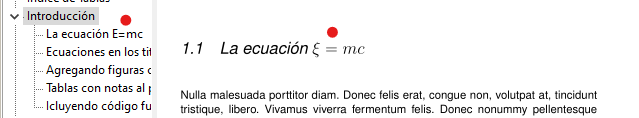
\includegraphics{ecuacionE-mc}
  }%
  \caption[Resultado del uso del comando texorpdfstring]{Resultado del uso del comando \mintinline{latex}{\texorpdfstring}.}
  \label{fig:texorpdf}
\end{figure}


\section[Código fuente en las secciones]{Código fuente en los titulos de las secciones}

Para escribir código fuente en los titulos de las \emph{secciones} utilizamos el paquete \mintinline{latex}{minted} el cual cargamos en el preambulo con el comando:

\mint{latex}{\usepackage{minted}}

Una vez cargado, podemos hacer uso del comando \mintinline{latex}{\mintinline{<language>}{<code>}}, donde \mintinline{latex}{<language>} lo sustituimos por el lenguaje que queremos utilizar, para este ejemplo utilizaremos \verb|latex|, y \verb|<code>| lo sustituimos por el código que queremos poner en linea con el texto. Un ejemplo de cómo se escribió la sección \ref{sec:texorpdf}:


\begin{minted}{latex}
  \section{Escribiendo ecuaciones en los titulos...
  de sección, sin errores, con el comando:\\
  \normalfont{\mintinline{latex}{\texorpdfstring{$<string>$}{<token>}}}}
\end{minted}

\lipsum[4] Revisar la tabla \ref{tab:apnx:uno:sec1} del Apéndice \ref{apnx:uno}.
\lipsum[5-6]\citep{Dan,Baz}.

\ref{sec:ecuacion}


\section[Agregando figuras]{Agregando figuras con el ambiente\\ \normalfont{\mintinline{latex}{figure}} y el comando \normalfont{\mintinline{latex}{\includegraphics}}}
% \normalfont{\texttt{includegraphics}}}% \texorpdfstring{$\si{km\per h = \si{m\per s}}$}{kmh-ms}}
\lipsum[7]

\begin{figure}[!ht]
  \center
  
\includegraphics[width=0.5\textwidth]{workinprogress}
  \caption{Figura de ejemplo.}
  \label{fig:ejemplo1}
\end{figure}

\lipsum[8]

\section{Citas en la descripción de figura}
\lipsum[9]
\begin{figure}[!ht]
  \center
  
\includegraphics[width=0.5\textwidth]{workinprogress}
  \caption[Figura de ejemplo numero 2]{Figura de ejemplo numero 2. Tomado de \citep{Dan}.}
  \label{fig:ejemplo2}
\end{figure}

Para lograr lo anterior se utilizó el siguiente código:
\begin{minted}{latex}
\begin{figure}[!ht]
  \center
  
\includegraphics[width=0.5\textwidth]{workinprogress}
  \caption[Figura de ejemplo numero 2]{Figura de ejemplo...
  numero 2. Tomado de \citep{Dan}.}
  \label{fig:ejemplo2}
\end{figure}
\end{minted}

Donde podemos observar que el comando \mintinline{latex}{\caption{...}}, tiene unos corchetes \verb|[...]| que anteceden a la descripción que contiene la cita, en estos corchetes se escribe un \emph{caption} opcional más corto y que no incluya ninguna cita. Con esto se corrigen errores de compilación.

\begin{table}[!ht]
  \caption{Tabla de ejemplo.}
  \centering
  \begin{tabular}{ccc}

    \toprule
    \textbf{Columna 1} & \textbf{Columna 2} & \textbf{Columna 3}\\
    \midrule
    Dato 1             & Dato 2             & Dato 3\\
    Dato 1             & Dato 2             & Dato 3\\
    Dato 1             & Dato 2             & Dato 3\\
    Dato 1             & Dato 2             & Dato 3\\
    Dato 1             & Dato 2             & Dato 3\\
    Dato 1             & Dato 2             & Dato 3\\
    Dato 1             & Dato 2             & Dato 3\\
    Dato 1             & Dato 2             & Dato 3\\
    \bottomrule

  \end{tabular}
  \label{tab:ejemplo1}
\end{table}

\lipsum[10]

\section[Tablas con notas al pie]{Tablas con notas al pie usando el paquete\\ {\normalfont\large\texttt{threeparttable}}}
\lipsum[11]


\begin{table}[!ht]
  \caption{Tabla de ejemplo.}
  \centering
  \begin{threeparttable}
  \begin{tabular}{ccc}

    \toprule
    \textbf{Columna 1} & \textbf{Columna 2}\tnote{a} & \textbf{Columna 3}\\
    \midrule
    Dato 1             & Dato 2             & Dato 3\\
    Dato 1             & Dato 2             & Dato 3\\
    Dato 1             & Dato 2             & Dato 3\\
    Dato 1             & Dato 2             & Dato 3\\
    Dato 1             & Dato 2             & Dato 3\\
    Dato 1             & Dato 2             & Dato 3\\
    Dato 1             & Dato 2             & Dato 3\\
    Dato 1             & Dato 2             & Dato 3\tnote{b}\\
    \bottomrule

  \end{tabular}
  \begin{tablenotes}
    \item \emph{Nota:} Esta es una nota al final de la tabla usando el paquete {\small\texttt{threeparttable}} y utilizando símbolos con el paquete {\small\verb|siunitx|} como \si{\degree}$C$.
    \item [a] Esta referencia es de la columna 2.
    \item [b] Este dato es 3.
  \end{tablenotes}
  \end{threeparttable}
  \label{tab:ejemplo4}
  \end{table}


\begin{table}[!ht]
  \caption{En un lugar de La Mancha.}
  \centering
  \begin{tabular}{ccc}

  \toprule
  \textbf{Don Quijote} & \textbf{Columna 2} & \textbf{Columna 3}\\
  \midrule
  Dato 1             & Dato 2             & Dato 3\\
  Dato 1             & Dato 2             & Dato 3\\
  Dato 1             & Dato 2             & Dato 3\\
  Dato 1             & Dato 2             & Dato 3\\
  Dato 1             & Dato 2             & Dato 3\\
  Dato 1             & Dato 2             & Dato 3\\
  Dato 1             & Dato 2             & Dato 3\\
  \bottomrule

  \end{tabular}
  \label{tab:quijote}
\end{table}


\begin{table}[!ht]
  \caption{Don Quijote de La Mancha.}
  \centering
  \begin{threeparttable}
  \begin{tabular}{ccc}

  \toprule
  \textbf{La Mancha}\tnote{a} & \textbf{Columna 2} & \textbf{Columna 3}\\
  \midrule
  Dato 1             & Dato 2             & Dato 3\\
  Dato 1             & Dato 2             & Dato 3\\
  Dato 1             & Dato 2             & Dato 3\\
  Dato 1             & Dato 2             & Dato 3\\
  Dato 1             & Dato 2             & Dato 3\\
  Dato 1             & Dato 2             & Dato 3\\
  \bottomrule

  \end{tabular}
  \begin{tablenotes}
    \item[a] En un lugar de La Mancha.
  \end{tablenotes}
  \end{threeparttable}
  \label{tab:donquijote}
\end{table}


\section{Icluyendo código fuente}
Este es un ejemplo de código python en línea con el texto texto texto y más texto:

{\small\mint{python}{import numpy as np}}

Y aquí un ejemplo de código latex en línea con el texto:

{\small\mint{tex}{\documentclass[12pt,towside]{book}}}
{\small\mint{tex}{\usepackage[utf8]{inputenc}}}
